\documentclass[aspectratio=169,obeyspaces,spaces,hyphens,dvipsnames]{beamer}
\usepackage[utf8x]{inputenc}
\usepackage{lmodern}% http://ctan.org/pkg/lm
\usepackage{minted}
\usepackage{hyperref}
\usepackage{xcolor}
\usepackage{pgfplots}
\usepackage{tikz}
\usepackage[normalem]{ulem}
\usepackage{textcomp}
\usepackage{marvosym} % \MVRIGHTarrow
\usepackage{tabularx}
%\usepackage{multimedia}

\mode<presentation>
\usetheme{INSA}

\def\signed #1{{\leavevmode\unskip\nobreak\hfil\penalty50\hskip2em
  \hbox{}\nobreak\hfil(#1)
  \parfillskip=0pt \finalhyphendemerits=0 \endgraf}}

\newsavebox\mybox
\newenvironment{aquote}[1]
  {\savebox\mybox{#1}\begin{quotation}}
  {\signed{\usebox\mybox}\end{quotation}}

\authors{Mylène Josserand}
\conference{Cours INSA}
\email{josserand.mylene@gmail.com}
\slidesurl{}

\title{Introduction à Linux embarqué}
\author[Mylène Josserand]
{Mylène Josserand}
\date[Octobre 2019]
{Cours INSA, Octobre 2019}
\institute[Bootlin]

\begin{document}

\begin{frame}
  \titlepage
\end{frame}

\begin{frame}{Mylène Josserand}
  \begin{itemize}
  \item Master pro génie physiologique et informatique, option Imagerie Médicale
  \item Ingénieure Kernel Linux et formatrice chez Bootlin
  \item Développement de driver Linux, intégration système sous Yocto Project/Open Embedded et Buildroot
  \item \url{josserand.mylene@gmail.com}
  \item Mylene sur IRC et MyleneJ sur github
  \end{itemize}
\end{frame}

\begin{frame}{Sommaire}
  \hspace{5cm}\tableofcontents
\end{frame}

%%%%%%%%%%%%%%%%%%%%%%%%%%%%%%%%%%%%%%%%%%%%%%
\section{Généralités}
%%%%%%%%%%%%%%%%%%%%%%%%%%%%%%%%%%%%%%%%%%%%%%

 \begin{frame}{Naissance de logiciel libre}{}
  \begin{itemize}
  \item 1983: Richard Stallman - Projet \textbf{GNU} et concept de logiciel libre. Developpement de gcc, gdb, glibc, etc
  \item 1991: Linus Torvalds - Projet noyau (\textbf{kernel}) \textbf{Linux}. De type Unix
  \item 1995: Linux est de plus en plus populaire sur les serveurs
  \item 2000: Linux est de plus en plus populaire sur les \textbf{systèmes embarqués}
  \item 2008: Linux est de plus en plus populaire sur les appareils mobiles
  \item 2010: Linux est de plus en plus populaire sur les téléphones
  \end{itemize}
\end{frame}

\begin{frame}{Logiciel libre ?}{}
  \begin{itemize}
  \item Un logiciel est considéré libre quand sa license respecte ces \textbf{4 libertés}:
    \begin{itemize}
    \item Liberté d'\textbf{éxécuter} le logiciel pour n'importe quel but
    \item Liberté d'\textbf{étudier} le logiciel et de le \textbf{modifier}
    \item Liberté de \textbf{redistribuer} des copies
    \item Liberté de \textbf{distribuer} des copies modifiées
    \end{itemize}
  \item Le code doit être disponible, le logiciel peut être modifié et distribué aux utilisateurs
  \end{itemize}
  \center\textbf{Parfait pour les systèmes embarqués !}
\end{frame}

\begin{frame}{Historique de Linux}{}
  \begin{itemize}
  \item Créé par Linus Torvalds en 1991
  \item Est un noyau : logiciel gérant les ressources d'une machine
  \item N'est pas un système d'exploitation : est lié au projet GNU\\
    \MVRightarrow{} distribution GNU/Linux
  \end{itemize}
    \center 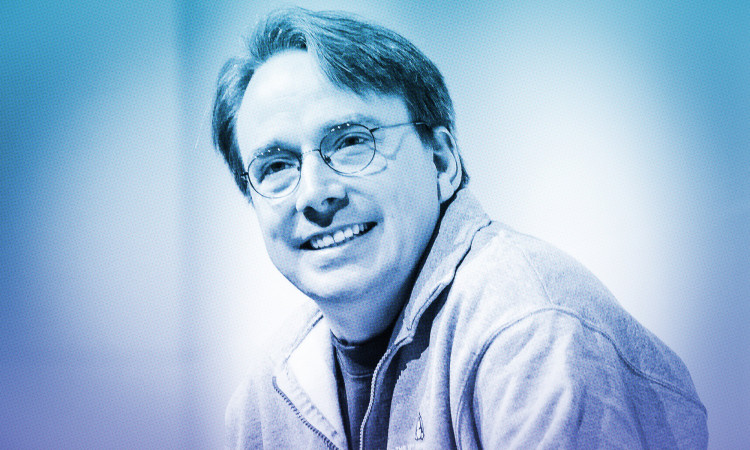
\includegraphics[height=0.3\textheight]{pictures/torvalds.jpg}
\end{frame}

\begin{frame}{Linux dans l'industrie}{}
  L'intérét pour les entreprises est:
  \begin{itemize}
  \item de maitriser les sources de leur OS
  \item d'économiser le prix des licences
  \item de bénéficier du support d'une communauté importante de développeur
  \item d'utiliser des composants déjà existants et testés par X personnes
  \end{itemize}
  Seule la partie Desktop a du mal face à ses concurrents
 \end{frame}

\subsection{Concepts}

\begin{frame}{Basé sur UNIX}{}
  \begin{itemize}
  \item Implémentation libre d'UNIX diffusé sous licence GPL
  \begin{center}
    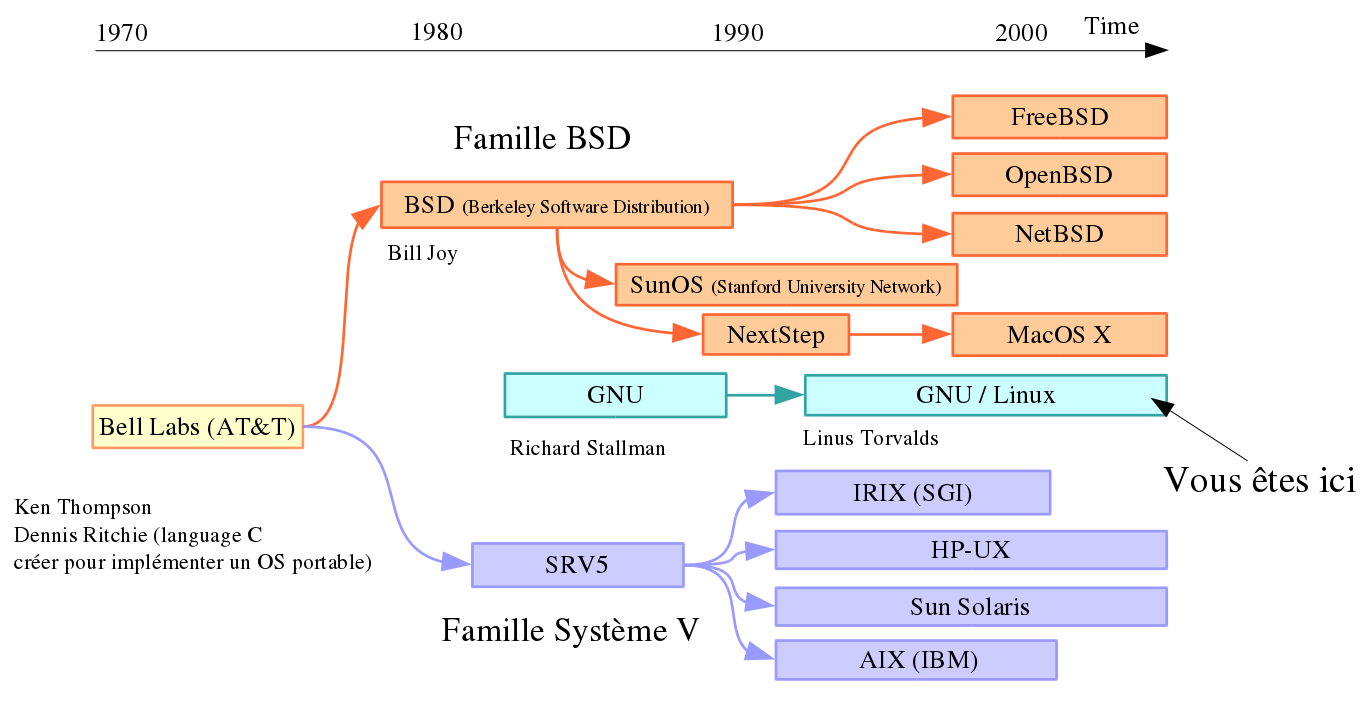
\includegraphics[height=0.4\textheight]{pictures/unix.png}
  \end{center}
  \item Les principes d'UNIX sont respectés:
  \begin{itemize}
  \item Simplicité, modularité, respect des standards, ouverture
  \item Abstraction du système : noyau = matériel ; userspace = applications
  \item Le noyau permet d'accéder au matériel (pilotes, appels système)
  \item Tout composant est un \textbf{fichier}: répertoire, périphérique, élément de communication, etc. (organisation arborescente)
  \item Puissance de la "ligne de commande" (shell et regexpr)
  \end{itemize}
  \end{itemize}
\end{frame}

\begin{frame}{Architecture}{}
  \begin{center}
    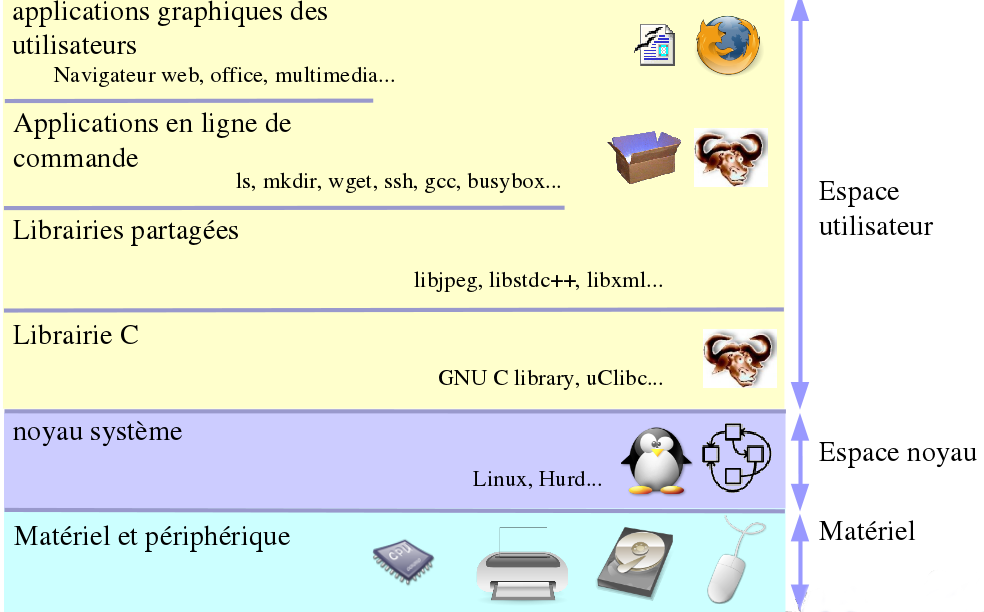
\includegraphics[height=0.8\textheight]{pictures/architecture-unix.png}
  \end{center}
\end{frame}

\begin{frame}{Fonctionnalitées}{}
  \begin{itemize}
  \item Noyau monolithique (en un seul fichier) + modules dynamiques
  \item Création des processus via fork() et exec()
  \item Multi-threading
  \item Nombreuses piles réseau (IPv4, IPv6, Ethernet, etc.)
  \item Organisation des fichiers arborescente à partir de la racine (/), montage et démontage logique (mount)
  \item Multi-utilisateurs avec un super-utilisateur (root) et des groupes
  \end{itemize}
\end{frame}

\subsection{Licence}

\begin{frame}{GPL en bref}{}
  \begin{itemize}
  \item GPL General Public License
  \item On la surnomme également copyleft
  \item La GPL v2 (1991) est la plus répandue (ex: noyau Linux)
  \item La licence s'applique uniquement en cas de redistribution
  \item Un code source utilisant du code GPL est du travail dérivé et doit être publié
  \item Publication: celui qui reçoit la version binaire peut obtenir le code source
  \item Pas de lien (ld) possible entre du code GPL et du code propriétaire
  \end{itemize}
\end{frame}

\begin{frame}{LGPL}{}
  \begin{itemize}
  \item La GPL est complexe à gérer dans l'industrie \MVRightarrow{} création de la LGPL
  \item Le lien avec du code propriétaire est possible avec la LGPL (Lesser/Library GPL) !
  \item En majeure partie, les bibliothèques système sont diffusées sous LGPL (exemple: GNU-libc)
  \item Dans le cas d'une application propriétaire il faut donc vérifier qu'aucune bibliothèque liée n'est GPL
  \item Le lien dynamique n'affranchit pas de la licence sauf dans des cas très particuliers
  \end{itemize}
\end{frame}

\begin{frame}{GPL uniquement pour LINUX}{}
  \begin{itemize}
  \item Dans l'espace noyau (pilotes), SEULE la GPL s'applique (en théorie) !
  \item En théorie: On ne peut utiliser les headers du noyau Linux pour créer des binaires non GPL
  \item Certaines fonctions ne sont pas disponibles si la licence n'est pas GPL
  \item En pratique: tolérance si le pilote n'a pas été créé pour Linux (cas du portage) \MVRightarrow{} nVidia, Broadcom, ...
  \item Cependant les pilotes binaires posent des soucis techniques vu qu'un pilote fonctionne pour la version de noyau utilisée pour la compilation
  \end{itemize}
\end{frame}

\begin{frame}{GPL V3}{}
  \begin{itemize}
  \item Nouvelle version sortie en 2007
  \item Oblige à fournir les éléments pour construire un logiciel fonctionnel \MVRightarrow{} réponse à la Tivoisation
  \item La GPL v2 demande uniquement la publication des sources à celui qui a reçu le binaire
  \item La GPL v3 ne sera pas utilisée pour le noyau Linux
  \item Voir: http://www.gnu.org/licenses/quick-guide-gplv3.fr.html
  \end{itemize}
\end{frame}

%%%%%%%%%%%%%%%%%%%%%%%%%%%%%%%%%%%%%%%%%%%%%%
\section{Architecture GNU/Linux}
%%%%%%%%%%%%%%%%%%%%%%%%%%%%%%%%%%%%%%%%%%%%%%

\begin{frame}{Système GNU/Linux}{}
  \begin{itemize}
  \item Noyau libre semblable à un noyau Unix
  \item Le système complet se repose sur les outils GNU:
    \begin{itemize}
    \item bibliothèque C, gcc, binutils, fileutils, make, emacs...
    \item Le système complet est donc appelé "\textbf{GNU / Linux}"
    \end{itemize}
  \item Très tôt partagé comme Logiciel Libre (Licence GPL) \MVRightarrow contributeurs et des utilisateurs de plus en plus nombreux
  \item Maintenant, fournit en tant que "distribution" (Ubuntu, Fedora, Debian, etc)
  \item Système entier composé de:
    \begin{itemize}
    \item Un bootloader (Rares sont les cartes capable de booter un noyau Linux)\\
      Il est trop gros et doit etre chargé en RAM. Elle doit etre initialisée par un microcode avant \MVRightarrow{} Utilité du \textbf{bootloader}
    \item Le noyau Linux qui gére les ressources de la machine
    \item Un système de fichier contenant à minima un programme de démarrage (rootfs)
    \end{itemize}
  \end{itemize}
\end{frame}

\begin{frame}{Noyau}{}
  \begin{itemize}
  \item Le noyau Linux est un binaire de type ELF
  \item Son image est souvent compressée pour gagner en taille lors du déploiement et de la copie en RAM
  \item Il contient un auto extracteur qui va le décomprésser
  \item Fournit des services nécéssaires à sa fonction:
    \begin{itemize}
    \item ordonanceur
    \item gestion mémoire, disque, interface réseaux
    \item service abtraits (systeme de fichier, pile réseaux ...)
    \end{itemize}
  \item Une grande partie du noyau peut etre déporté en \textbf{module} chargé dynamiquement
  \end{itemize}
\end{frame}

\begin{frame}{Architecture}{Noyau}
  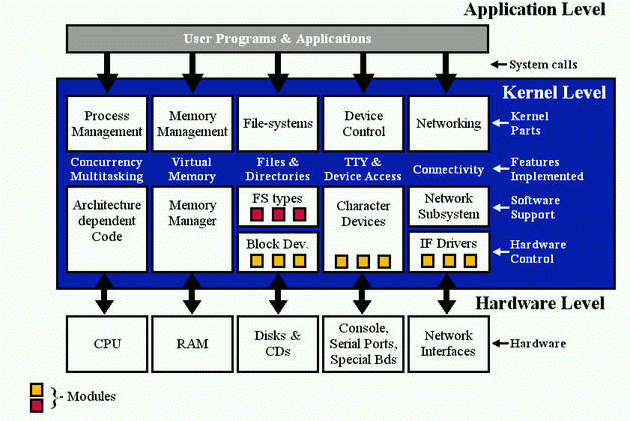
\includegraphics[width=10cm]{pictures/kernel_arch.png}
\end{frame}

\begin{frame}{Module noyau}
  \begin{itemize}
  \item Modules noyau: .ko (Kernel Object)
  \item Les modules binaires sont liés à la version du noyau !
  \item Peut se compiler après mais nécessite les entetes du noyau
  \item Mécanisme système pour charger les modules dynamiquement: modprobe, insmod, rmmod
  \end{itemize}
\end{frame}

\begin{frame}{Organisation d'un rootfs}
  \begin{itemize}
  \item Organisation commune à 90\% entre les UNIX
  \item Quelques spécificités GNU/Linux et distribution
  \item Tout commence depuis la racine \texttt{/}
  \item Puis, organisation en dossier/sous-dossier:
    \begin{itemize}
    \item \texttt{/bin,/sbin,/usr/bin,/usr/sbin}: binaires communs et systèmes
    \item \texttt{/lib,/usr/lib}: bibliothèques et modules noyau
    \item \texttt{/etc}: fichiers de configuration
    \item \texttt{/dev}: nœuds d'accès aux périphériques
    \item \texttt{/var}: fichiers variables comme log, mail, ...
    \item \texttt{/opt}: pour les programmes externes (ex: LibreOffice)
    \item \texttt{/home}: accueille les répertoires des utilisateurs
    \end{itemize}
  \end{itemize}
\end{frame}

\begin{frame}{Organisation d'un rootfs}
  \begin{itemize}
  \item Quelques répertoires spéciaux:
    \begin{itemize}
    \item \texttt{/lib/modules}: contient les modules du noyau
    \item \texttt{/root}: home-directory de l'utilisateur root
    \item \texttt{/media}: point de montage des volumes amovibles
    \item \texttt{/proc}: système de fichier virtuel (état du système)
    \item \texttt{/sys}: idem pour les périphériques connectés
    \item \texttt{/boot}: noyau statique (vmlinuz, uImage, ...)
    \end{itemize}
  \end{itemize}
\end{frame}

\begin{frame}{/proc}
  \begin{itemize}
  \item Système de fichier virtuel (lecture/écriture) géré par le noyau. (Réponse sur solicitation, pas d'écriture sur un support)
  \item Intérêt: manipuler les variables systèmes comme de fichiers (cat, echo, grep)
  \item Exemples:
    \begin{itemize}
    \item \texttt{/proc/version}: version du noyau
    \item \texttt{/proc/cpuinfo}: type(s) de processeur(s)
    \item \texttt{/proc/interrupts}: interruptions
    \item \texttt{/proc/pid}: répertoire décrivant le processus associé au pid
    \item \texttt{/proc/mounts}: partitions montées
    \item \texttt{/proc/modules}: liste des modules noyau chargés
    \end{itemize}
  \item Nombreuses commandes systèmes basées sur \texttt{/proc} : lsmod, lspci, top, mount, ...
  \end{itemize}
\end{frame}

\begin{frame}{/sys}
  \begin{itemize}
  \item Introduit dans le noyau 2.6 (2003) \MVRightarrow{} sysfs
  \item Vue synthétique des périphériques connectés
    \begin{itemize}
    \item \texttt{/sys/class}
    \item \texttt{/sys/modules}
    \item \texttt{/sys/bus}
    \end{itemize}
  \item But: mieux gérer l'ajout/suppression dynamique des périphériques (hotplug)
  \item Utilisé par UDEV pour créer dynamiquement les entrées dans \texttt{/dev}
  \item Quelques recouvrements avec /proc (bus PCI, USB, ...)
  \end{itemize}
\end{frame}

\section{Execution d'un système GNU/Linux}

\begin{frame}{Démarrage}
  \begin{columns}
    \column{0.6\textwidth}
    \begin{enumerate}
    \item Le matériel lance le bootloader
    \item Le bootloader configure la RAM et le support contenant le noyau
    \item Le bootloader copie le noyau en RAM et lui donne la main
    \item Le noyau s'auto extrait en RAM
    \item Le noyau initialise les périphériques et les sub-systèmes (ordonnanceur, pile réseaux, sytème de fichier,...)
    \item Le noyau récupère dans le rootfs le binaire d'initialisation (\texttt{/sbin/init} par défaut) et crée le processus 1
    \item Ce processus est chargé de démarrer tous les services en espaces utilisateurs
    \end{enumerate}
    \column{0.4\textwidth}
    \begin{center}
      \includegraphics[height=0.7\textheight]{graphics/overall-boot-sequence.pdf}
    \end{center}
  \end{columns}
\end{frame}

\begin{frame}{Le processus init}
  \begin{itemize}
  \item Le père des processus du système
  \item Plusieurs systèmes possibles:
    \begin{itemize}
    \item systemV:
      \begin{itemize}
      \item facile à configurer car basé sur des scripts shell
      \item architecture vieille et dépassé. Moins performant
      \end{itemize}
    \item systemd:
      \begin{itemize}
      \item Parallélise l'initialisation du système. Centralise de nombreux services (logs, etc)
      \item Plus complexe à prendre en main et moins modulaire pour certain
      \end{itemize}
    \item custom:
      \begin{itemize}
      \item Linux permet d'utiliser son propre binaire init
      \item Il faut gérer soit même le système
      \end{itemize}
    \end{itemize}
  \end{itemize}
\end{frame}

%%%%%%%%%%%%%%%%%%%%%%%%%%%%%%%%%%%%%%%%%%%%%%
\section{Introduction aux systèmes embarqués}
%%%%%%%%%%%%%%%%%%%%%%%%%%%%%%%%%%%%%%%%%%%%%%

\subsection{Systèmes embarqués}
\begin{frame}{Systèmes embarqués}
  \begin{itemize}
  \item Un système embarqué est un système concu pour ne réaliser qu'un certains nombre de tâches défini
  \item On associe un système à une fonction (ou un groupe de fonction)
  \item On cherche à maitriser le fonctionnement du système
  \item Différe des systèmes génériques censés savoir tout faire sur n'importe quelle plateforme
  \end{itemize}
\end{frame}

\begin{frame}{Exemples}
  \begin{tabular}{ccc}
    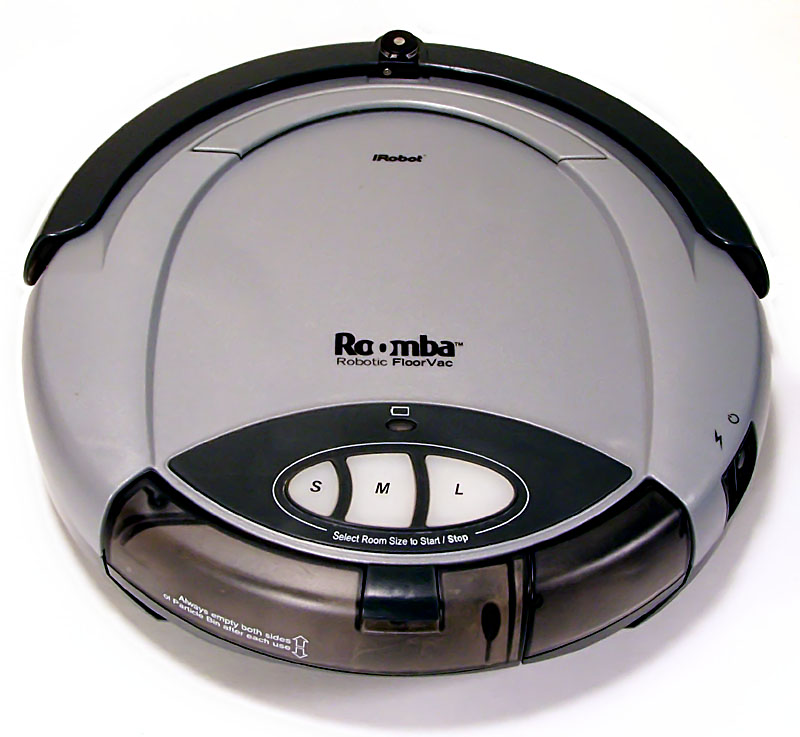
\includegraphics[height=2.5cm]{pictures/roomba.jpg} & \hspace{1.5cm}
    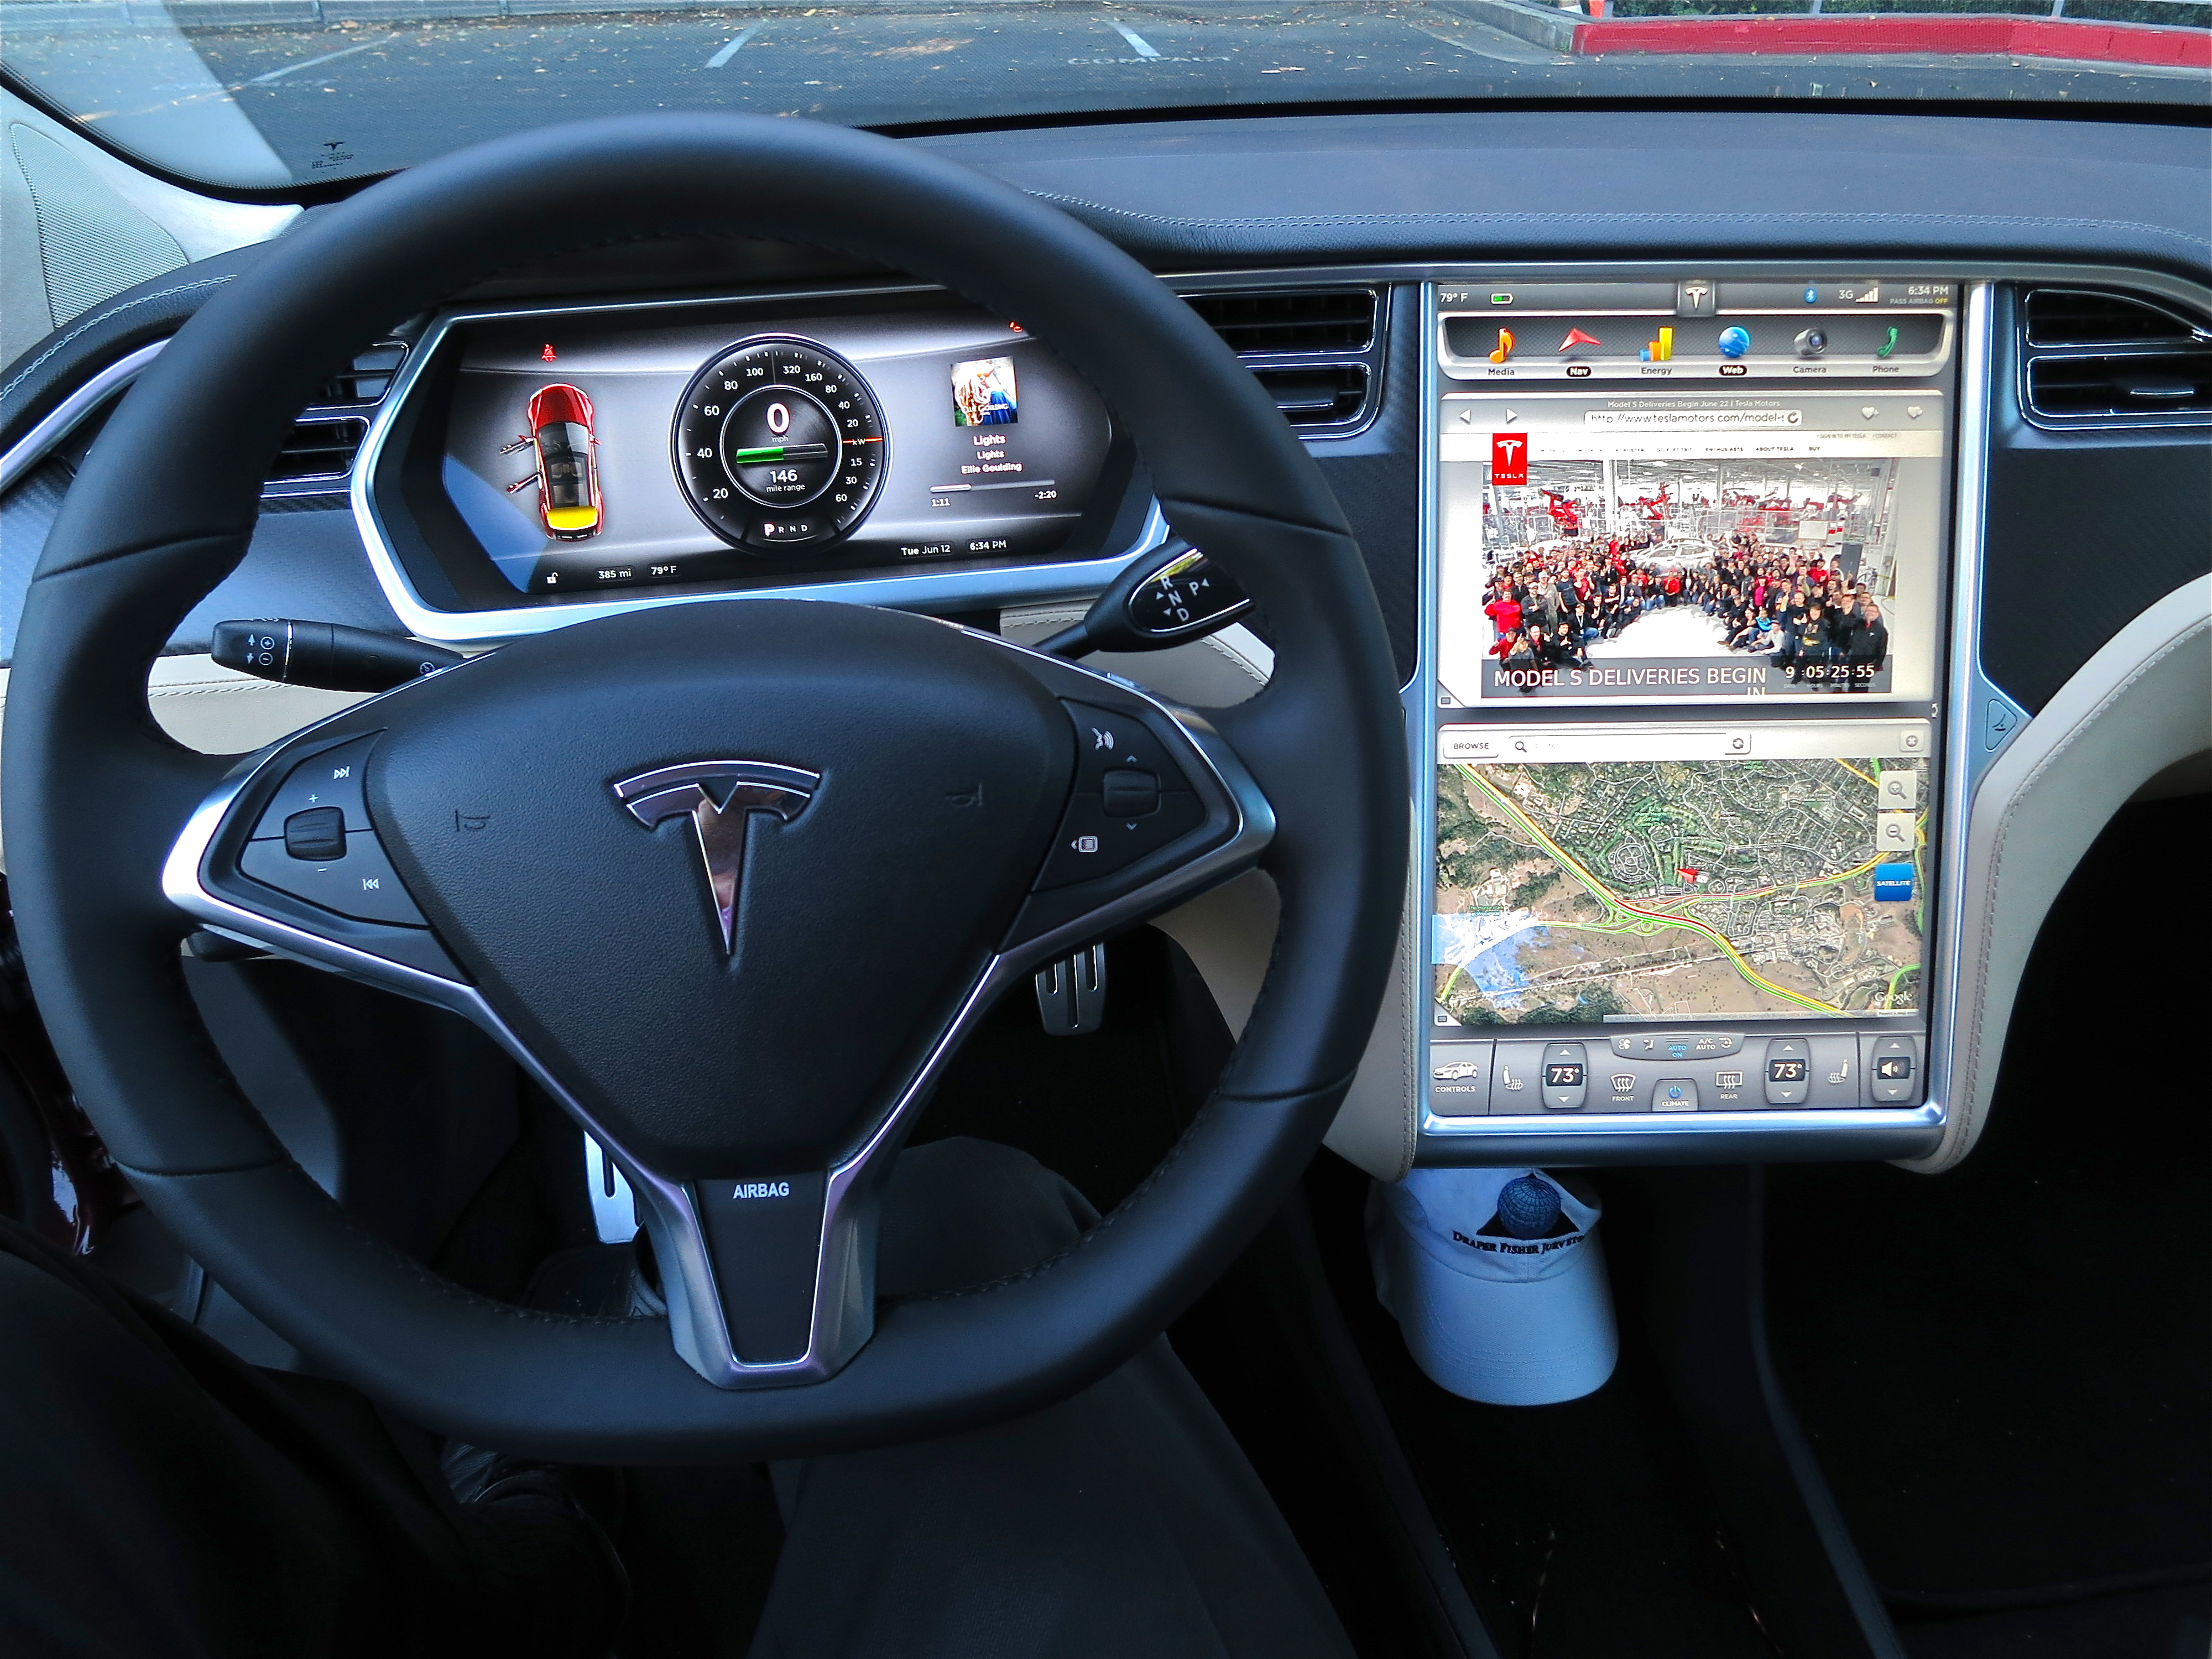
\includegraphics[height=2.5cm]{pictures/tesla.jpg} & \hspace{1.5cm}
    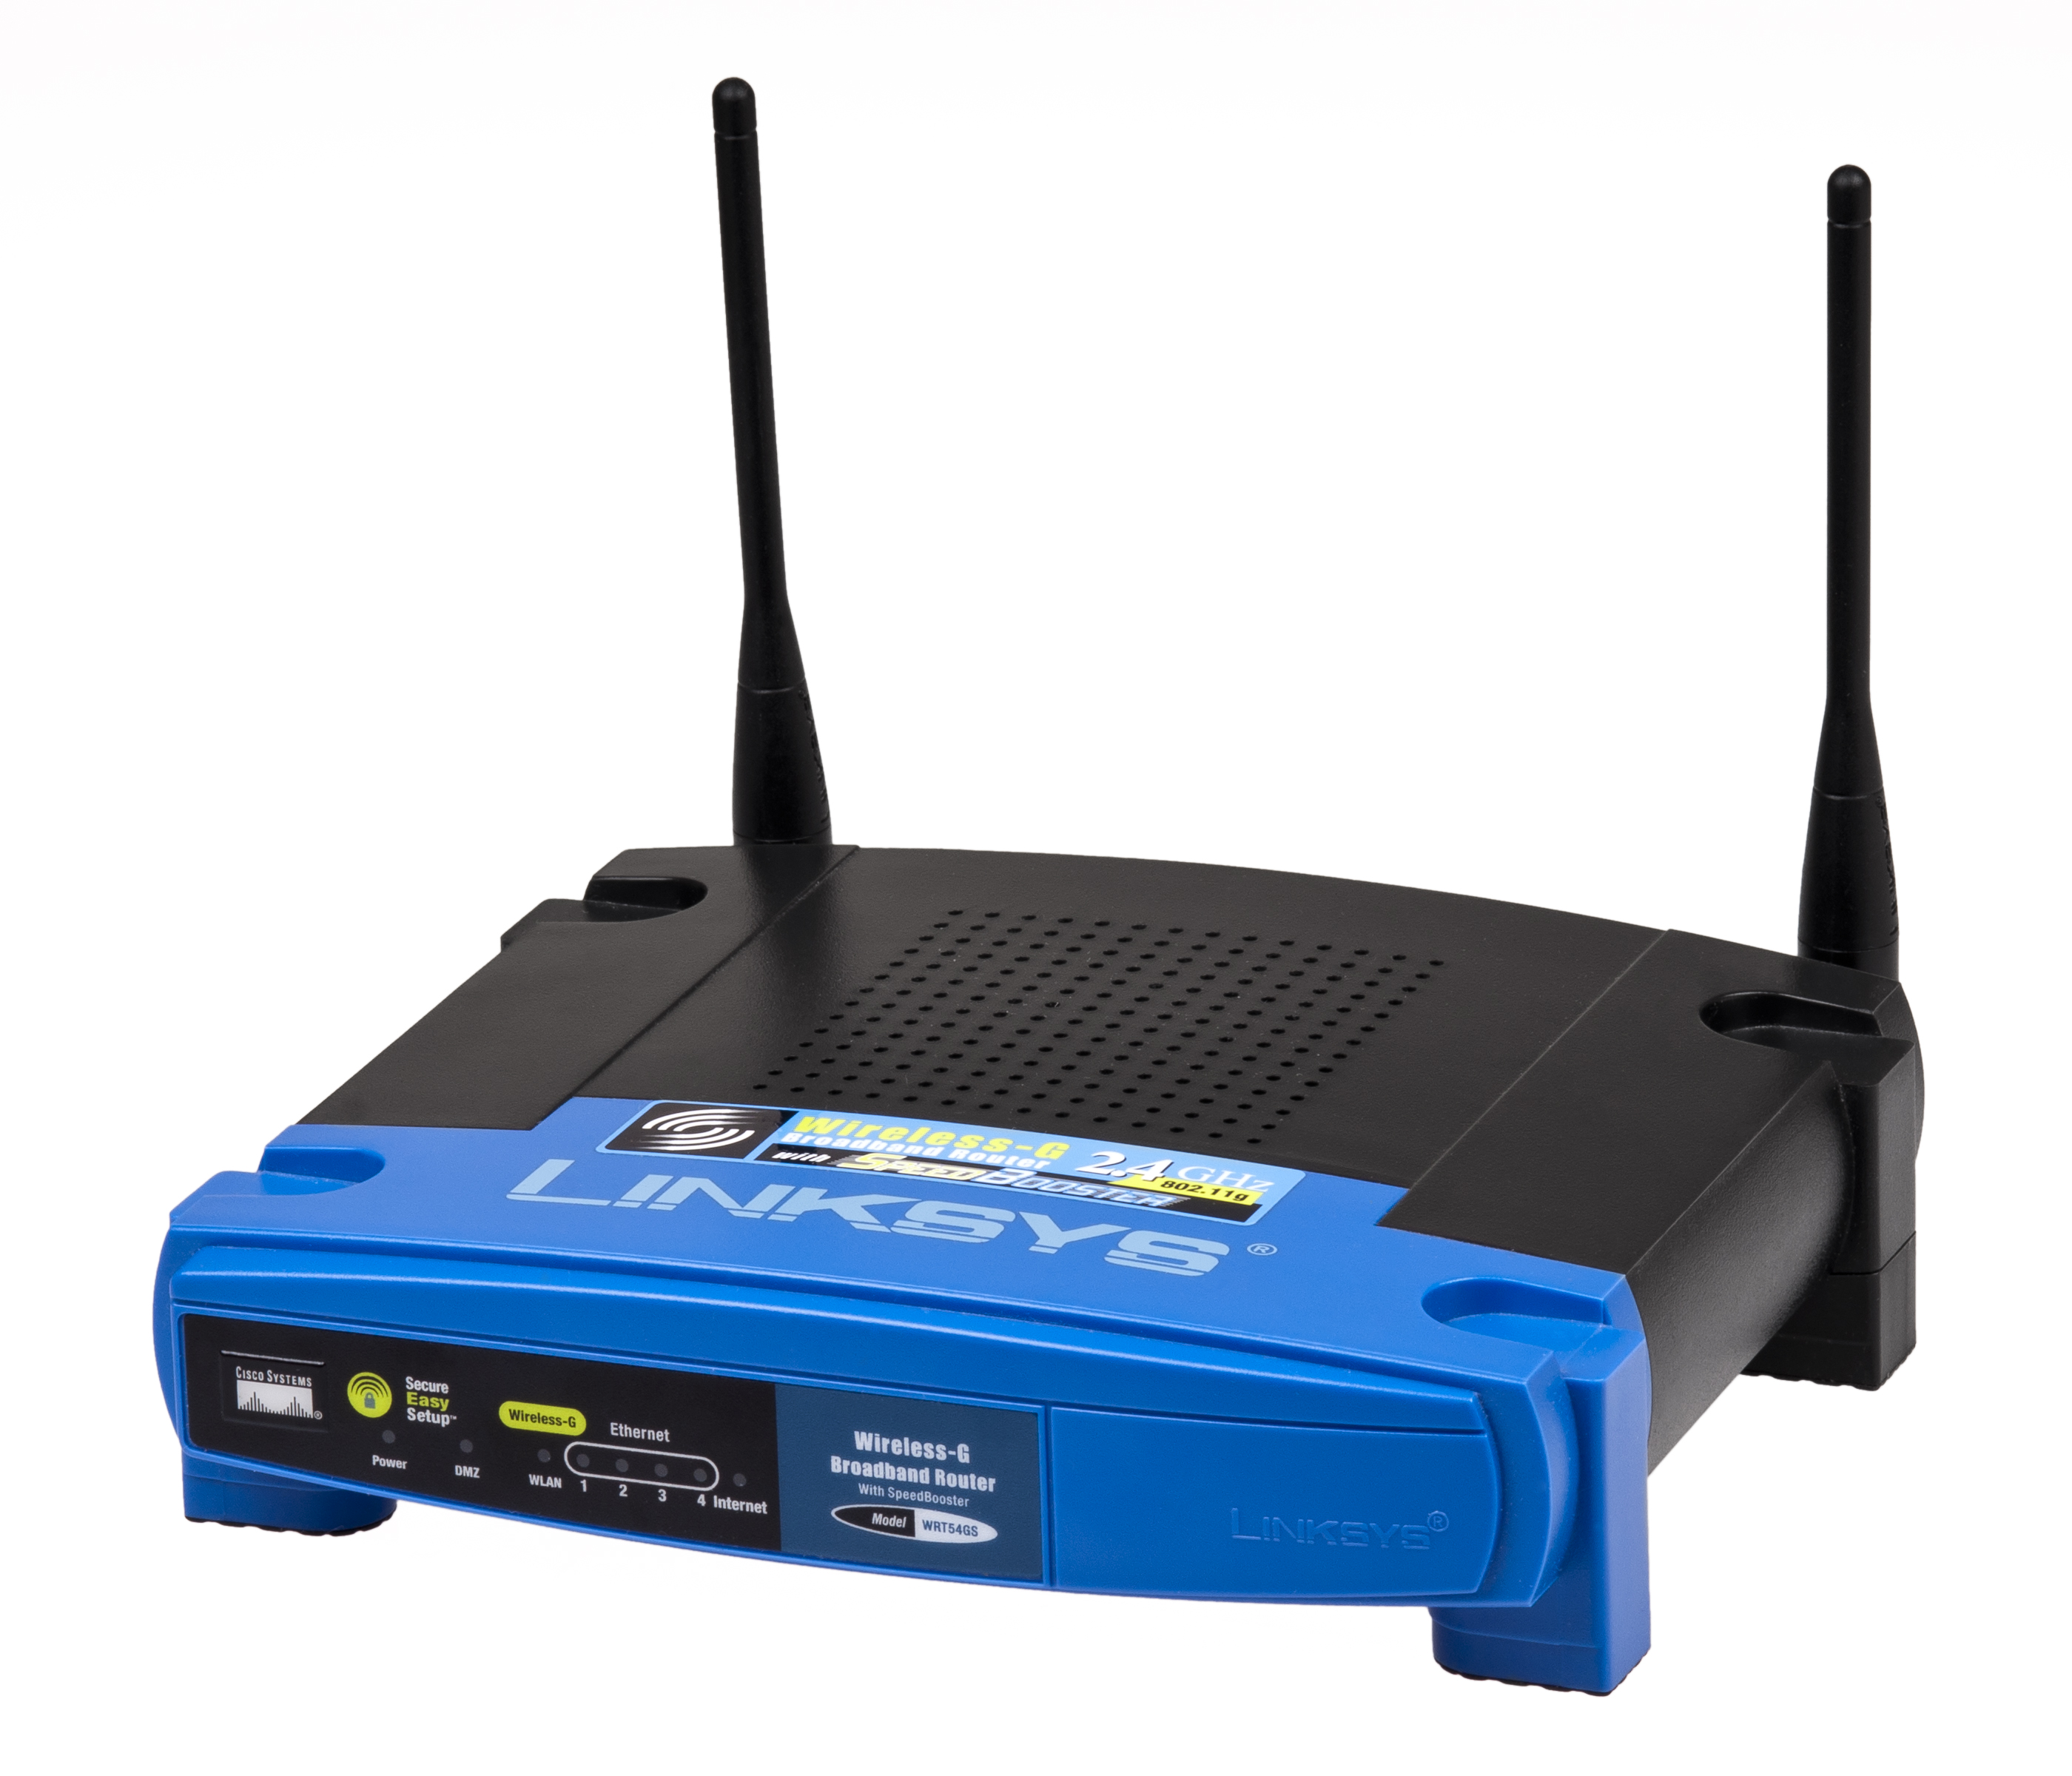
\includegraphics[height=2.5cm]{pictures/router.jpg}
  \end{tabular}
\end{frame}

\begin{frame}{Systèmes embarqués GNU/Linux?}
  \begin{itemize}
  \item Utilisé depuis longtemps comme serveur
  \item Pourquoi ne pas l'utiliser pour d'autres systèmes génériques?
  \item De nombreuses architectures supportées par Linux (ARM, mips, powerpc ...)
  \item Systèmes fiables et performants
  \item De nombreuses fonctionnalités déjà codées et validées
  \item Nécessite un BSP (Board support package) et un peu d'adaptation
  \end{itemize}
\end{frame}

\subsection{Eléments nécéssaires}
\begin{frame}{Eléments nécéssaires}
  \begin{itemize}
  \item Une système GNU/Linux embarqué nécéssite:
    \begin{itemize}
    \item Chaîne de compilation croisée (Gcc, as, ld, LibC)
    \item Un Bootloader (U-Boot, barebox, grub, isolinux)
    \item Noyau Linux adapté à l'archi hardware
    \item Outils GNU/LINUX Commandes Linux (sh, ls, cp, etc.)
    \item Applications ...
    \item Outil de génération (BR, OE, ...)
    \end{itemize}
  \end{itemize}
\end{frame}

%%%%%%%%%%%%%%%%%%%%%%%%%%%%%%%%%%%%%%%%%%%%%%
\section{Toolchain}
%%%%%%%%%%%%%%%%%%%%%%%%%%%%%%%%%%%%%%%%%%%%%%

\begin{frame}{Toolchain}{}
  \begin{itemize}
  \item Un point très complexe !
  \item Nécessité de construire une chaîne croisée :
    \begin{itemize}
    \item GCC
    \item Binutils (as, ld, ...)
    \item Dépendances avec le noyau (system calls, ...) \MVRightarrow erreur "Kernel too old"
    \item Choix d'une libC \MVRightarrow Glibc, uClibc, Eglibc, ...
    \item GDB
    \item Toute autre bibliothèque utilisée \MVRightarrow libstdc++
    \item Dépendances avec le compilateur hôte
    \end{itemize}
  \end{itemize}
\end{frame}

\begin{frame}{Toolchain}{}
  \begin{itemize}
  \item Interaction entre la libC et le noyau Linux
    \begin{itemize}
    \item Appels systèmes (nombre, définition)
    \item Constantes
    \item Structures de données, etc.
    \end{itemize}
  \item Compiler la libC – et certaines applications - nécessite les en-tête du noyau
  \item Disponibles dans \code{<linux/...>} et \code{<asm/...>} et d'autres répertoires des sources du noyau (include, ...)
  \end{itemize}
\end{frame}

\subsection{Compilateur binaire}
\begin{frame}{compilateur binaire}
  \begin{itemize}
  \item Utiliser un compilateur binaire :
    \begin{itemize}
    \item ELDK: \url{http://www.denx.de/wiki/DULG/ELDK}
    \item Code Sourcery : \url{https://www.mentor.com/embedded-software/sourcery-tools-services/}
    \item Linaro Toolchain \url{https://www.linaro.org/downloads/}
    \item Bootlin's toolchains: \url{https://toolchains.bootlin.com}
    \item Installation simple
    \item Support (payant) possible
    \item Configuration connue \MVRightarrow support par les forums
    \end{itemize}
  \item Par contre:
    \begin{itemize}
    \item Versions des composants figées
    \item Non utilisation des possibilitées du CPU
    \item Choix libC limité
    \end{itemize}
  \end{itemize}
\end{frame}

\subsection{Compilateur source}
\begin{frame}{Compilé son compilateur}
  \begin{itemize}
  \item Construire un compilateur:
    \begin{itemize}
    \item Crosstool \MVRightarrow obsolète
    \item Crosstool-NG \MVRightarrow assez complexe à prendre en main
    \item Buildroot / OpenEmbedded
    \end{itemize}
  \item Aucun n'est "plug and play"
  \item La mise au point peut prendre des jours, voire plus !
  \item Binaires produits : arm-linux-* (gcc, as, ld, ar, nm, ...)
  \end{itemize}
\end{frame}

%%%%%%%%%%%%%%%%%%%%%%%%%%%%%%%%%%%%%%%%%%%%%%
\section{Construire son système embarqué}
%%%%%%%%%%%%%%%%%%%%%%%%%%%%%%%%%%%%%%%%%%%%%%

\begin{frame}{Architecture}{}
  \begin{center}
    \includegraphics[height=0.8\textheight]{graphics/linux-system-architecture.pdf}
  \end{center}
\end{frame}

\subsection{Bootloader}
\begin{frame}{Bootloader}{}
  \begin{itemize}
  \item Premier logiciel lancé au démarrage de la machine
  \item Initialise le matériel (RAM, stockage, ...) nécésaire au boot
  \item Charge le noyau en RAM et lui donne la main
  \item Permet de donner des arguments au noyau
  \item Exemples:
    \begin{itemize}
    \item U-boot (supporte de nombreux architectures, la référence)
    \item Barebox (u-boot v2, meilleure archi, moins de fonctionnalités pour l'instant)
    \item grub (x86, serveur et desktop principalement)
    \item isolinux (alternative x86 à grub)
    \end{itemize}
  \item Un système embarqué nécéssitera une configuration et un support matériel dans le bootloader.
  \end{itemize}
\end{frame}

\subsection{Kernel}
\begin{frame}{Kernel}{}
  \begin{itemize}
  \item Génération d'un noyau:
    \begin{enumerate}
    \item Récupération du noyau (kernel.org)
    \item Développement du support des drivers manquants
    \item Création du support de la carte (board config  3.10 device tree)
    \item Configuration le noyau (make menuconfig)
    \item Compilation du noyau (make uImage)
    \item Installation sur la cible
    \end{enumerate}
  \item Binaire utilisable dans arch/arm/boot/zImage ou bien arch/arm/boot/uImage (pour U-Boot)
  \item Binaire vmlinux utile pour le debug
  \item Utilisation des variables ARCH et CROSS\_COMPILE.
  \end{itemize}
\end{frame}

\subsection{Rootfs}
\begin{frame}{Binaires de base}{}
  \begin{itemize}
  \item Binaires de base indispensables au système (ls, bash, dd, top, cp, mv, init,...)
  \item Trois possibilités:
    \begin{itemize}
    \item Récupérer les sources et les compiler un par un. (laborieux)
    \item GNU/Linux coreutils (trop lourd pour l'embarqué)
    \item Busybox (regroupe la majorité des commandes Linux en un seul executable)
      \begin{itemize}
      \item 95\% des distributions Linux embarqués l'utilise
      \item Simple, léger, portable
      \item Diffusé sous licence GPLv2
      \end{itemize}
    \end{itemize}
  \end{itemize}
\end{frame}

\begin{frame}{Busybox}{}
  \begin{itemize}
  \item Utilisation des variables ARCH et CROSS\_COMPILE. (comme le noyau)
  \item Génération de busybox:
    \begin{enumerate}
    \item Récupération des sources
    \item Configuration (make menuconfig)
    \item Compilation (make uImage)
    \item Installation sur la cible (make CONFIG\_PREFIX=... install)
    \end{enumerate}
  \end{itemize}
\end{frame}

\begin{frame}{Rootfs - Peuplement}
  \begin{itemize}
  \item Peuplement d'un rootfs:
    \begin{enumerate}
    \item Installation de la libc et des autres librairies fournies par la toolchain
    \item Installation des binaires de busybox
    \item Création de la configuration de démarrage (/etc/init.d)
    \item Ajout des nodes dans /dev (si pas de mécanisme automatique)
    \item Ajout des librairies et applications du projet.
    \end{enumerate}
  \item Deux méthodes:
    \begin{itemize}
    \item A la main, copier ou installer chaque fichier/logiciel manuellement. (LFS) \MVRightarrow Inenvisageable à moyen et long terme
    \item Automatiser soit en scriptant soit en utilisant un système existant (OE, yocto, buildroot, uclinux ...) \MVRightarrow Plus rapide et plus sûr. Indispensable en production pour maitriser son livrable.
    \end{itemize}
  \end{itemize}
\end{frame}

%%%%%%%%%%%%%%%%%%%%%%%%%%%%%%%%%%%%%%%%%%%%%%
\section{Mise au point}
%%%%%%%%%%%%%%%%%%%%%%%%%%%%%%%%%%%%%%%%%%%%%%

\subsection{BSP}
\begin{frame}{BSP}{}
  \begin{itemize}
  \item Une plateforme "neuve" nécessite des ajustements pour fonctionner:
    \begin{itemize}
    \item Adaptation de la toolchain
    \item Support des drivers dans le \textbf{bootloader} et le \textbf{kernel}
    \item Ajout des fonctionnalités dans le bootloader et le kernel (réseau, NAND, HDD, ...)
    \end{itemize}
  \item Fourni par le constructeur de la plateforme électronique.
  \item Si on est le constructeur, il faut développer le support.
  \item Outils à disposition (gdb, sonde JTAG, ftrace, oscilloscope, multimetre ...)
  \end{itemize}
\end{frame}

\subsection{User space}
\begin{frame}{User space}{}
  \begin{itemize}
  \item Lorsque le BSP est OK, la mise au point en espace utilisateur peut commencer
  \item De nombreux outils permettent de mettre au point des applications:
    \begin{itemize}
    \item printf: outil simple à mettre en oeuvre et connu de tout le monde
    \item syslog: utile pour vérifier le bon fonctionnement ou détecter des anomalies
    \item valgrind: vérifie la bonne utilisation de la mémoire
    \item strace/ltrace: affiche les appels systèmes et librairies
    \item gdb: debugguer GNU/LINUX
      \begin{itemize}
      \item permet d'acceder à la memoire, controler l'execution, monitoré les threads ...
      \item gdbserver pour les cibles embarqués pour déporter le debug
      \end{itemize}
    \end{itemize}
  \end{itemize}
\end{frame}

%%%%%%%%%%%%%%%%%%%%%%%%%%%%%%%%%%%%%%%%%%%%%%
\section{Les build-systèmes}
%%%%%%%%%%%%%%%%%%%%%%%%%%%%%%%%%%%%%%%%%%%%%%

\begin{frame}{Les différents travails en Linux embarqué}
  \begin{itemize}
  \item {\bf BSP}: portage du bootloader et du noyau Linux + développement de drivers.
  \item {\bf Integration système}: assembler tous les composents userspace nécessaires pour le système, les configurer, mécanismes de mise à jour, etc
  \item {\bf Développement applicatif}: écrire des applications ou librairies spécifiques à l'entreprise
  \end{itemize}
\end{frame}

\begin{frame}{Complexité de l'intégration userspace}
  \begin{center}
    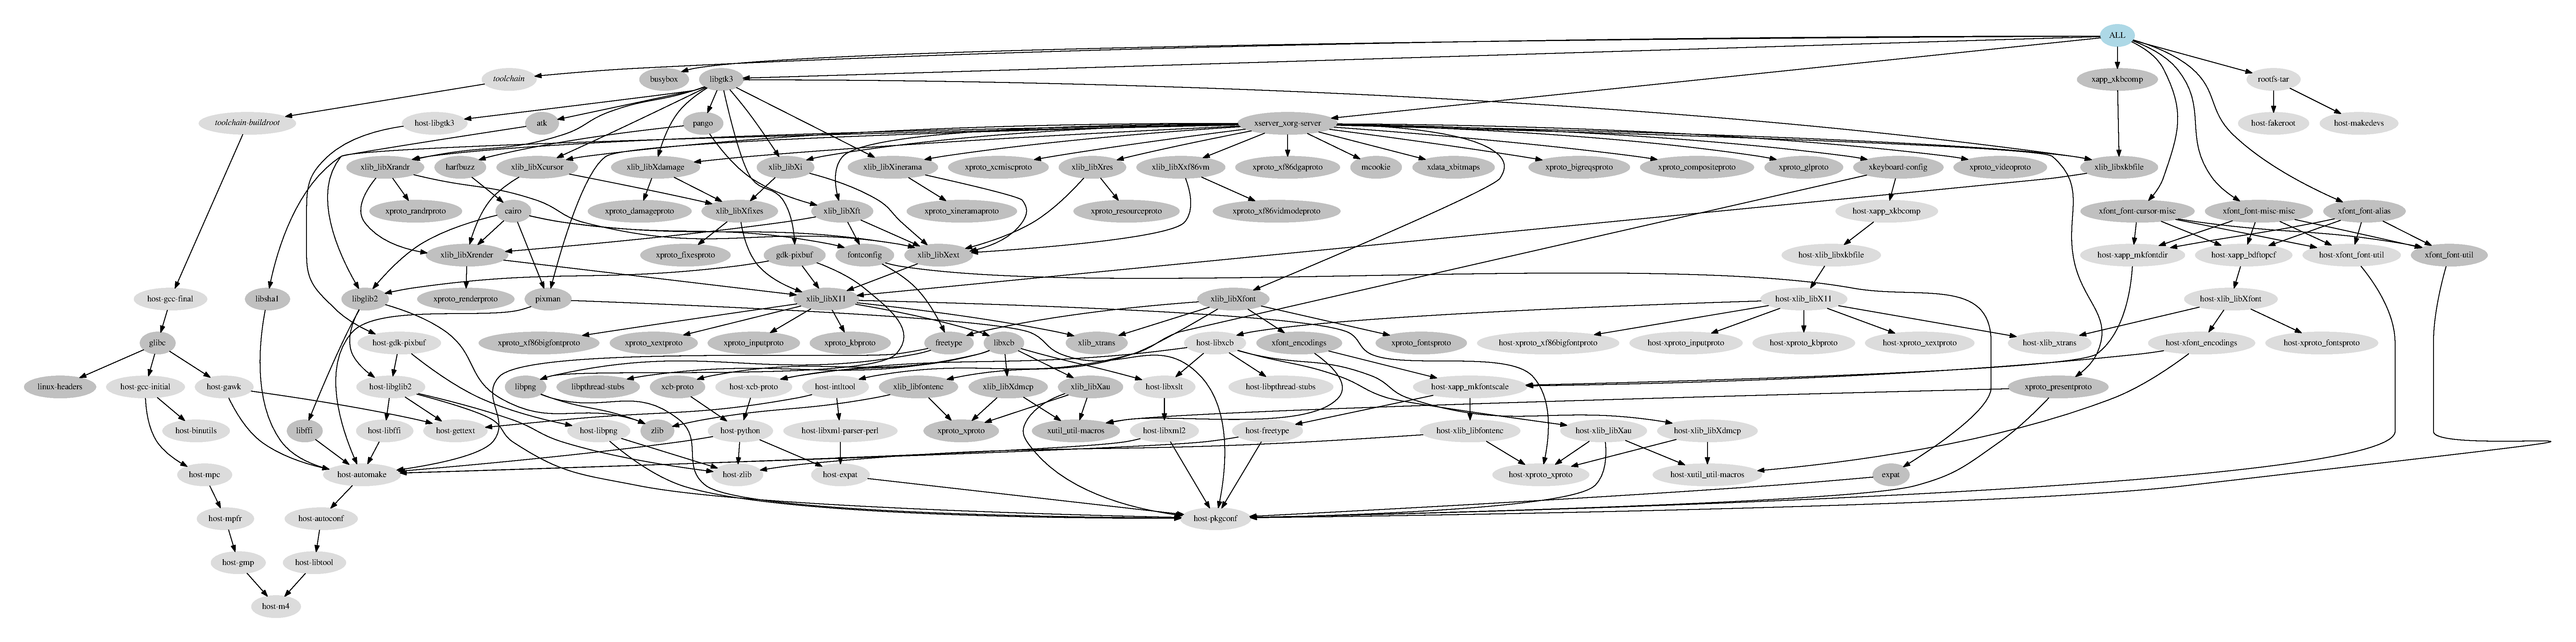
\includegraphics[width=\textwidth]{graphics/graph-depends.pdf}
  \end{center}
\end{frame}

\begin{frame}{Intégration système: plusieurs possibilités}
  \tiny
  \begin{tabularx}{14cm}{|X|X|X|}
    \hline
    & {\bf Pros} & {\bf Cons} \\
    \hline
    {\bf Compiler tout manuellement} &
    Complètement flexible \newline
    Gagne en expérience &
    Enfer des dépendances \newline
    Doit comprendre tout un tas de détails \newline
    Compatibilité des versions \newline
    Manque de reproductibilité \\
    \hline
    {\bf Distributions binaires} \newline Debian, Ubuntu, Fedora, etc.
    &
    Facile à créer et étendre
    &
    Difficile à customiser \newline
    Difficile à optimizer (temps de boot, taille) \newline
    Difficile de compiler depuis les sources \newline
    Système gros \newline
    Compilation native \newline
    Pas de mécanisme bien définis pour générer une image \newline
    Pleins de dépendances obligatoires \newline
    Pas disponibles pour toutes les architectures \\
    \hline
    {\bf Systèmes de build} \newline Buildroot, Yocto, PTXdist, etc.
    &
    Quasiment complètement flexible \newline
    Compile depuis les sources : customisation et optimisation faciles \newline
    Complètement reproductible \newline
    Cross-compilation \newline
    Contains des paquets spécifique à l'embarqué \newline
    &
    Pas aussi facile qu'une distribution binaire \newline
    Temps de build \\
    \hline
  \end{tabularx}
\end{frame}

\begin{frame}{Build system: principe}
  \begin{center}
    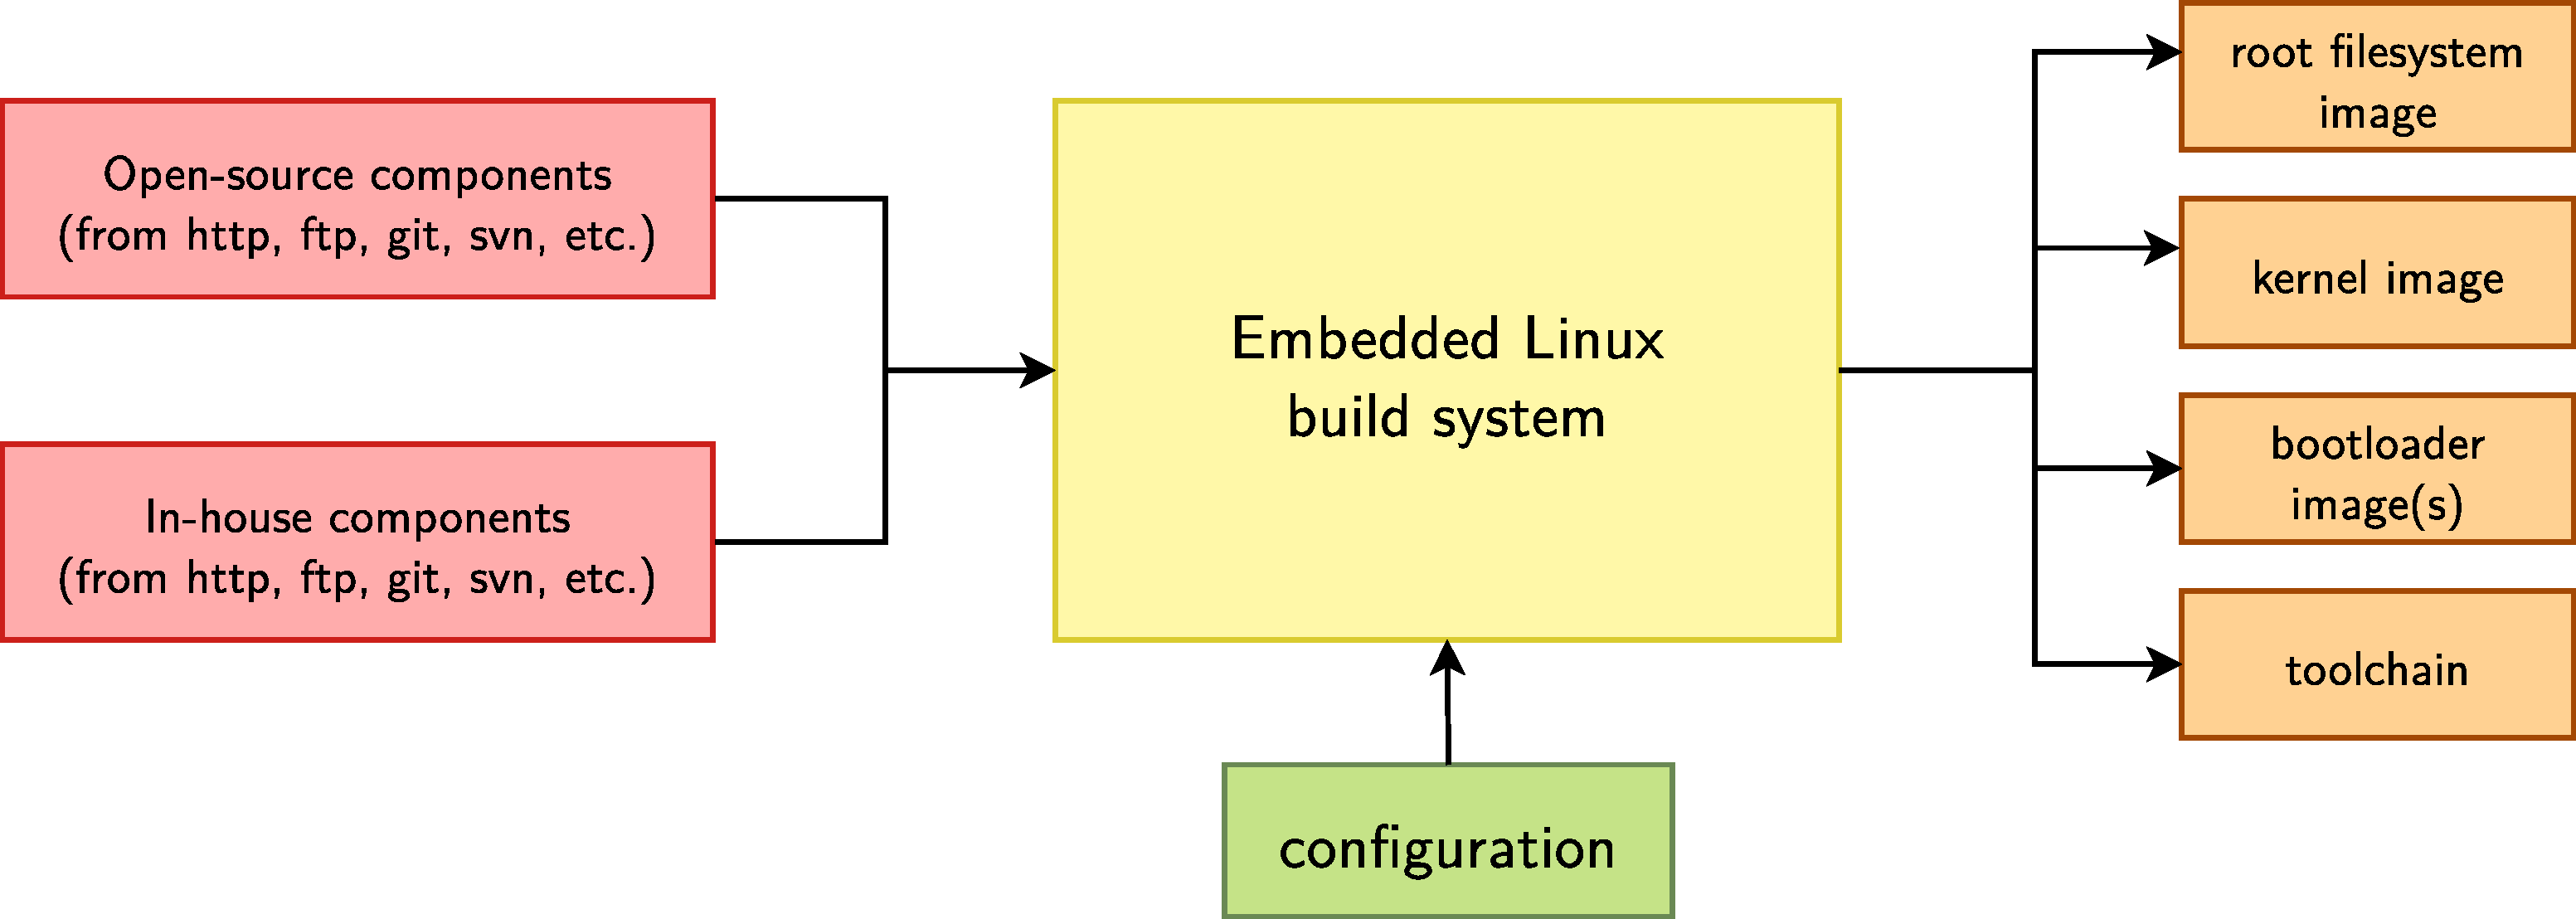
\includegraphics[width=0.9\textwidth]{graphics/buildsystem-principle.pdf}
  \end{center}
  \begin{itemize}
  \item Compilation depuis les sources $\rightarrow$ flexibilité
  \item Cross-compilation $\rightarrow$ rapidité à compiler si utilise des machines de build
  \item Recettes pour compiler des composants $\rightarrow$ facile
  \end{itemize}
\end{frame}

\begin{frame}{Les outils}
  \begin{itemize}
  \item Beaucoup de solutions possibles : Yocto/OpenEmbedded, PTXdist,
    Buildroot, OpenBricks, OpenWRT, etc.
  \item Mais 2 solutions émergent comme les plus populaires :
    \begin{itemize}
    \item {\bf Yocto/OpenEmbedded}\\Compile une distribution Linux complète avec des paquets binaires. Très puissant mais complexe et prend beaucoup de temps à apprendre
    \item {\bf Buildroot}\\Compile une image de rootfs, pas de paquets binaires. Beaucoup plus simple à utiliser, comprendre et modifier.
    \end{itemize}
  \end{itemize}
\end{frame}

%%%%%%%%%%%%%%%%%%%%%%%%%%%%%%%%%%%%%%%%%%%%%%
\section{Introduction à Buildroot}
%%%%%%%%%%%%%%%%%%%%%%%%%%%%%%%%%%%%%%%%%%%%%%

\begin{frame}{Buildroot}
  \begin{itemize}
  \item Peut compiler une toolchain, un rootfs, un kernel, un bootloader
  \item {\bf Facile à configurer}: menuconfig, xconfig, etc.
  \item {\bf Rapide}: compile un rootfs en quelques minutes
  \item Facile à comprendre: écrit en make, bonne documentation
  \item {\bf Petit}: root filesystem, débute en 2 MB
  \item {\bf 2200+ paquets} pour userspace
  \item {\bf Pleins d'architectures} supportées
  \item {\bf Technologies bien connues}: {\em make} et {\em kconfig}
  \item Neutre
  \item Communauté active, releases régulières
  \item \url{https://buildroot.org}
  \end{itemize}
\end{frame}

\begin{frame}{Buts dans le design}
  \begin{itemize}
  \item Buildroot est designé avec des buts précis:
    \begin{itemize}
    \item Simple à utiliser
    \item Simple à personnaliser
    \item Builds \textbf{reproductibles}
    \item Petit root filesystem
    \item Temps de build relativement rapide
    \item Facile à comprendre
    \end{itemize}
  \item Pas toutes les fonctionnalités possibles supportées
  \item Plus compliqués et avec beaucoup de fonctionnalités : Yocto Project, OpenEmbedded
  \end{itemize}
\end{frame}

\begin{frame}{Buildroot dans l'industrie?}
  \begin{columns}
    \column{0.6\textwidth}
    \begin{itemize}
    \item {\bf Entreprises}
      \begin{itemize}
      \item Google
      \item Barco
      \item Rockwell Collins
      \end{itemize}
    \item {\bf Vendeurs de processors}
      \begin{itemize}
      \item Imagination Technologies
      \item Marvell
      \item Microchip (Atmel)
      \item Analog Devices
      \end{itemize}
    \item {\bf Vendeur de SoM et de cartes}
    \item Beaucoup d'entreprises lors de {\em R\&D} sur des produits
    \item Beaucoup de {\bf hobbyists} des cartes de developpement :
      Raspberry Pi, BeagleBone Black, etc.
  \end{itemize}
  \column{0.4\textwidth}
  \only{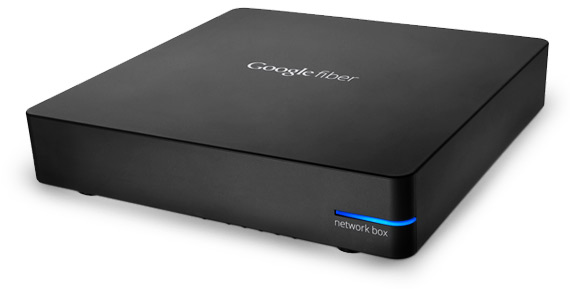
\includegraphics[height=0.25\textheight]{pictures/google-fiber-box.jpg}}\\
  \only{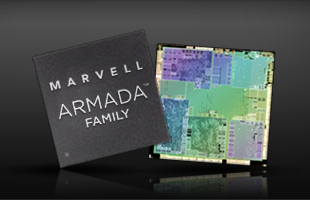
\includegraphics[height=0.25\textheight]{pictures/armada.jpg}}\\
  \only{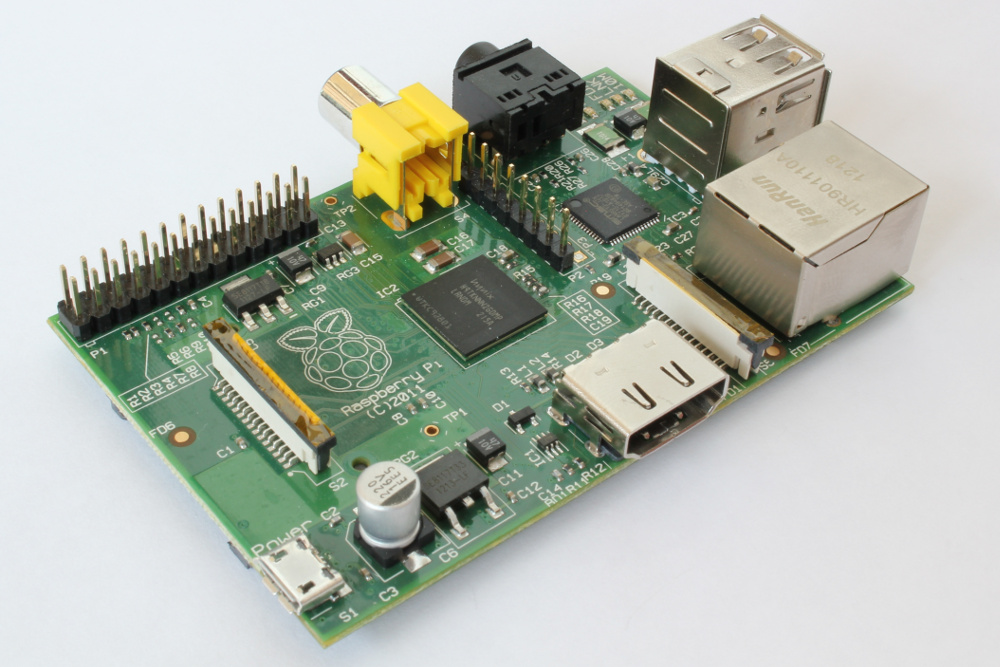
\includegraphics[height=0.25\textheight]{pictures/raspberrypi.jpg}}
  \end{columns}
\end{frame}

\begin{frame}{Buildroot}
  \begin{itemize}
  \item Releases stables tous les 3 mois:
    \begin{itemize}
    \item \code{YYYY.02}, \code{YYYY.05}, \code{YYYY.08},
      \code{YYYY.11}
    \end{itemize}
  \item Archives disponibles pour chaque release stable
    \begin{itemize}
    \item \url{https://buildroot.org/downloads/}
    \end{itemize}
  \item Plus pratique via git
    \begin{itemize}
    \item Visualisation de ses modifications
    \item Simplification des contribution
    \item \code{git clone git://git.busybox.net/buildroot}
    \item Tags git disponible pour chaque release stable
    \end{itemize}
  \item Une {\bf long term support (LTS)} release chaque année
    \begin{itemize}
    \item Maintenue durant 1 an
    \item Fixes de sécurité, bugs, compilation, etc
    \item LTS actuelle : \code{2019.02}
    \end{itemize}
  \end{itemize}
\end{frame}

\begin{frame}[fragile]{Utilisation de Buildroot}
  \begin{itemize}
  \item Implémenté via \code{make}
    \begin{itemize}
    \item Avec quelques shell scripts d'aide
    \end{itemize}
  \item Toutes les interactions via \code{make} dans le répertoire principal de Buildroot
    \begin{block}{}
\begin{verbatim}
$ cd buildroot/
$ make help
\end{verbatim}
    \end{block}
  \item Pas besoin d'être \code{root}, désigné pour être exécuté avec privilèges utilisateurs
    \begin{itemize}
    \item Executer en root est même fortement découragé!
    \end{itemize}
  \end{itemize}
\end{frame}

\begin{frame}{Configuration de Buildroot}
  \begin{itemize}
  \item Comme le kernel Linux, utilise {\em Kconfig}
  \item Un choix des interfaces de configuration :
    \begin{itemize}
    \item \code{make menuconfig}
    \item \code{make nconfig}
    \item \code{make xconfig}
    \item \code{make gconfig}
    \end{itemize}
  \item Vérifier que les librairies nécessaires sont installées
    ({\em ncurses} pour menuconfig/nconfig, {\em Qt} pour xconfig, {\em
      Gtk} pour gconfig)
  \end{itemize}
\end{frame}

\begin{frame}{Main {\tt menuconfig} menu}
  \begin{center}
    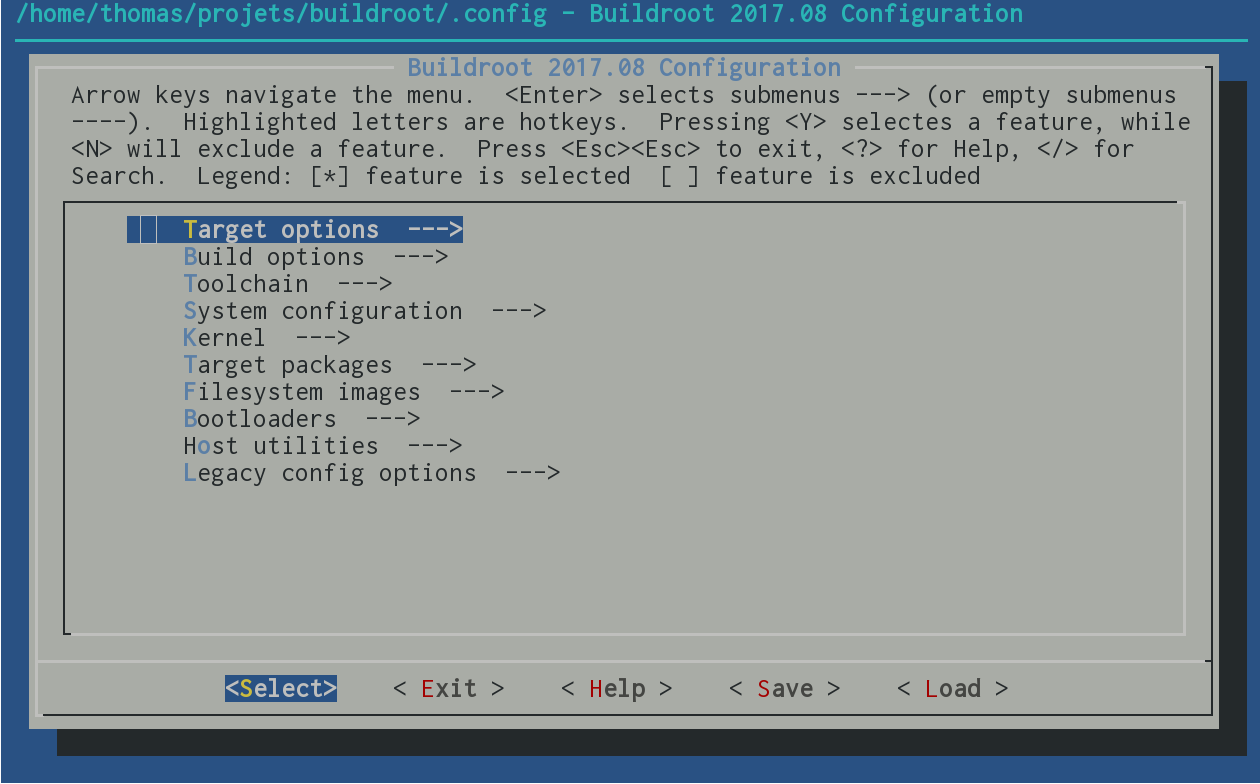
\includegraphics[height=0.8\textheight]{pictures/menuconfig.png}
  \end{center}
\end{frame}

\begin{frame}[fragile]{Lancer une compilation}
  \begin{itemize}
  \item Aussi simple que:
    \begin{block}{}
\begin{verbatim}
$ make
\end{verbatim}
    \end{block}
  \item Si veut garder un log de la compilation pour analyse ou investigation:
    \begin{block}{}
\begin{verbatim}
$ make 2>&1 | tee build.log
\end{verbatim}
    \end{block}
  \end{itemize}
\end{frame}

\begin{frame}{Résultats de compilation}
  \begin{itemize}
  \item Localisé dans \code{output/images}
  \item Selon la configuration, le répertoire contiendra:
    \begin{itemize}
    \item Une ou plusieurs images de root filesystem dans des formats différents
    \item Une image kernel, un ou plusieurs Device Tree blobs
    \item Une ou plusieurs images de bootloader
    \end{itemize}
  \item Pas de standard pour installer les images sur une carte
    \begin{itemize}
    \item Trop spécifiques à la carte
    \item Buildroot fournit des outils pour générer une image de carte SD / clef USB
      ({\em genimage}) ou de flasher directement sur certaines plateformes :
      SAM-BA pour Microchip, imx-usb-loader pour i.MX6, OpenOCD, etc.
    \end{itemize}
  \end{itemize}
\end{frame}


\begin{frame}
  \begin{center}
    \Huge
    Merci de votre attention ! \\
    Questions ? Commentaires ?\\
    \vspace{1cm}
    \large
    Mylène Josserand — \code{josserand.mylene@gmail.com}\\
    \vspace{1cm}
    Slides under CC-BY-SA 3.0\\
    © Copyright 2004-\the\year, Bootlin\\
    \scriptsize
    \url{https://github.com/MyleneJ/cours-insa}
  \end{center}
\end{frame}

\end{document}
